\documentclass{article}
\usepackage{amsthm}
\usepackage{comment}
\usepackage{mathbbol}

\theoremstyle{definition}
\newtheorem{definition}{Definition}
\usepackage[skip=4pt]{caption}
\usepackage{graphicx}
\usepackage{xcolor}
\usepackage{hyperref}
\usepackage{graphicx}
\usepackage{float}
\usepackage{amsmath}
\usepackage{relsize}
\usepackage{listings}

\usepackage[bibstyle=authoryear, style=numeric, citestyle=numeric-comp, backend=bibtex]{biblatex}
\bibliography{bibliography/krr,bibliography/procs,local}

% Begin Variables definition
\newcommand\widthimg{11cm}
% End Variables definition



\begin{document}

\title{\huge{Individual Research Module: Plan Merging}}

\author{
\\[1cm] \textbf{Supervisors}
\\[0.2cm] Klaus Strauch 
\\[0.2cm] Torsten Schaub
\\[0.2cm] Etienne Tignon
\\[3cm] Aurélien SIMON }

\maketitle
\thispagestyle{empty}

\pagenumbering{arabic} 


\newpage
\setcounter{page}{1}
\tableofcontents
\newpage
\listoffigures

\newpage

\section{Introduction}
Multi-Agent PathFinding or MAPF \cite{ststfekomawaliatcokubabo19a,ststfekomawaliatcokubabo19b,stern19a} for short, is a fundamental AI problem that has a wide-range real application: GPS, video-games, routing, planning, traffic control etc. In few words, consider agents moving in an environment, going from an initial to a goal position; MAPF is about finding a path for each agent, such as there is no collision between them. Multiple approaches exist; Search-algorithm (CBS \cite{shstfest15a}) or reduction solving based (\cite{barsva19a}). 
In this report we focus on an approach call ``Plan Merging'', this approach aims to solve MAPF problems by using two distinct steps; computing a set of paths for each agent independently (which correspond to classic pathfinding / single-agent pathfinding~\cite{foghkuhagu21a}). We will refer to this step as Individual Path Finding, in short IPF. The second step, to find a solution avoiding collision using the previously computed paths. Formalization of each step will be described in their respective sections. The interest in this approach is due to pathfinding complexity which is lower than MAPF complexity \cite{nebel19a}; the idea is then to use this property to expect saving computation time or space complexity. 
The approach in its definition is close to CBS, however, the planning part of CBS stops if a conflict occurs and re-iter the planning part considering the conflict previously encountered which is not the case for the IPF; the conflict handling would be in the merging section.
The work achieved tries to formally define these two steps but also tries to provide workflow and different approaches with their formal definitions. The report includes a background part which formally introduce the notion of MAPF and also some definitions and notions that will be used in the whole report. The report then includes the Individual Path Finding section describes formalization of different cost or objective function for paths such as, functions based on the intrinsic property of a path, functions based on the path in the graph and functions based on other agents paths. The report then describes formalization of Plan Merging by introducing a witness solver, definitions, heuristics and approaches. And then, finally conclude. 



\section{Background}\label{sec:background}

The following definitions of Multi-Agent Path Finding (MAPF) follow the ones in~\cite{husvobbass22a}. MAPF is a triple $(V,E,A)$ where \(V,E\) denotes a connected graph, \(V\) being a set of vertices and \(E\) a set of edges connecting them. Then \(A\) being a set of agents. For each agent \(a=(s,g) \in A\), \(s\) is a vertex in \(V\) denoting the starting location and \(g\) is also a vertex in \(V\) denoting the goal location. We consider that every starting position and every goal position are disjoint.
For each discrete time step \(t\in \mathbb{N}_0\), an agent can either; wait at its current vertex or move to a neighboring one.

The output for MAPF problems is a plan. A plan being a collection $(\pi_a)_{a\in A}$ of finite walks in $(V,E)$ where each walk $\pi_a$ is represented by a finite sequence of adjacent or identical vertices in $V$ from $s$ to $g$ for agent $a = (s,g)$. We use \(\pi_a (t) = v\) to denote that agent \(a\) is located at vertex \(v\) at time step \(t\). 
As consequences, for each \(a=(s,g) \in A\), we have $\pi_a(0) = s$ and  $\pi_a(|\pi_a|-1) = g$ (where $|\pi_a|$ gives the length of walk $\pi_a$). Generally, for any \(a=(s,g)\) and any $0 \leq t \leq |\pi_a|-1$, we have \(\pi_a(t) \in V\). In addition, we also have $(\pi_a(t),\pi_a(t+1))\in E$ with $0 \leq t < |\pi_a|-1$

A plan is considered as \textit{valid} if, taken pairwisely, walks are collision-free. A vertex conflict occurs whenever two different agents occupy the same vertex at the same time step. Formally, we have \(conflict(a,a',t)\) if given any $a,a'\in A$  and $t\in\mathbb{N}_0$, we have $\pi_a(t) = \pi_{a'}(t)$. An edge conflict (or swapping conflict) occurs whenever two agents exchange their position or are using the same vertex at the same time, which implies that edge conflict is defined on time step \(t\) and \(t-1\). We have \(conflict(a,a',t)\) if given any $a,a'\in A$  and $t\in\mathbb{N}_0$, we have $\pi_a(t-1) = \pi_{a'}(t)$ and $\pi_a(t) = \pi_{a'}(t-1)$.

A plan $(\pi_a)_{a\in A}$ has a conflict, if a conflict $(a, a',t)$ occurs in $(\pi_a)_{a\in A}$ for some pair $a,a'\in A$ of agents and a time step $t\in\mathbb{N}_0$.

\textit{Sum-of-costs} and \textit{makespan} of a plan $(\pi_a)_{a\in A}$ are respectively defined as such; $\sum_{a\in A} (|\pi_a| - 1)$ and $\max_{a\in A} (|\pi_a| - 1)$.


Furthermore, we also define in which MAPF problem specification the following work has been conducted. Since we would define object that require distance and/or coordinates such as rectangle or circles, we will consider that graphs have Cartesian coordinate system, which means we can represent them as a grid. In addition, we work on a non-anonymous MAPF variant with edge conflict and vertex conflict. 







\section{Individual Path finding}\label{sec:ipf}
This section describes functions that can be used as cost/objective function. This means it can be maximized, minimized in order to obtain paths with different properties.

\subsection{Formalization}

Individual Path Finding (IPF) aims to compute for each agent, a non-empty set of paths. IPF can be summarized as ``MAPF without collisions''; it takes the same input as MAPF (see \ref{sec:background}), it however differ on the output. The output is a triple \((V,E,\tau)\) where \(\tau\) is a set where the relation is bijective, considering an agent \(a \in A\), we have  \(\tau[a]\) being a non-empty set of path, we can refer to \(\tau[a]\) with \(\gamma\) or \(\gamma_a\) if necessary for better understanding or lighter notation. Let an agent \(a=(s,g)\), for any \(\pi\in \gamma_a\), \(\pi(0) = s\) and \(\pi(|\pi|-1) = g\). Thus, every paths composing \(\gamma\) can have a different length.


We will then list and classify what can be the different kind of paths that can compose \(\tau\), what are their properties, advantages and inconvenient.


We also define the \(pick\) function which allows lighter notation; \(pick\) takes as input a set of paths \(\gamma\) and returns one of the paths in \(\gamma\).




\subsection{Properties of a Path}

\subsubsection{Path of defined length}
A noticeable property is the \textbf{length} of the path, denoted as \(|\pi|\). We can distinguish two cases; the length is the minimal possible or it is strictly higher than the minimal. The first case gives us a lower bound for searching a solution, and if a solution exists using only shortest path, it is an optimal solution. In the second case optimality is no longer guarantee. However, working with path of defined length, combined with knowledge of the graph, it can make the ``field of action'' for the merging algorithm wider, which can result of finding a solution, but also rise the number of possibilities which can lead to more computing difficulties.


\begin{definition}[Shortest Path (SP)]\label{def:shortest_path}
  Given an initial and a final position, an associated path \(\pi\) is in the set \(SP\) if \(\pi\) is valid and no path \(\pi'\) such as \(|\pi| > |\pi'|\). Generally, \(SP\) the set of all of the shortest path possible for a given initial and final position. For lighter notation, \(|SP^i|\) to the size of  paths \(\pi\) composing \(SP\)
\end{definition}



\(2k\) paths are specific paths of defined length, they are of length \(|SP| + 2k\) where \(k\) is a positive integer. The \(2k\) section represents the fact that in order to ``resolve'' a conflict, if wait moves are not possible for any reason (specification, approaches, instance\ldots), solving a conflict would require at least two moves. This kind of paths comes with an assumption; computing an additional path of \(2k\) kind is (way) faster than trying to solve a conflict in the solver. Intuitively, this kind of paths can be quite interesting to solve~\nameref{def:blocking_agent} instances.





\subsubsection{Path containing bending(s)}

Counting bending in a path require to work on a graph using cartesian coordinate system. From coordinates we can compare angles of the vectors made from the current vertex and the previous one, to the current one and the next one. If angles are equals, it means that the path is continuing in its previous direction (angles have the same direction), otherwise a direction change is identified. Formally, we can define a bending in an cartesian coordinate system of the path \(\pi\) at time step \(t\) as such: \[
 u = \overrightarrow{(\pi(t-1),\pi(t))} \text{ and  } v = \overrightarrow{(\pi(t),\pi(t+1))}
\]
\[
  bending(\pi,t) = 
    \begin{cases}
      1  & \text{if }  \widehat{u} = \widehat{v} \\
      0  & \text{otherwise}
    \end{cases}  
\] Then, the number of bending in a path is \[
  Bending(\pi) =  \sum_{t=1}^{|\pi|-2}{bending(\pi,t)}
\] 

If a ``waiting'' move is considered as a vector of size 0, by definition, any vector of size 0 is ``perpendicular'' to any other one.

It is important to mention that approach for counting bendings makes sense for a grid scenario with defined and restricted directions; there high chance that bendings definition should be changed for scenarios working with continuous directions or a 3+ dimension. 
Given the number of bending, we can deduce information; with zero bending, we can trivially deduce that the initial position and the goal position are on the same column or row, furthermore the path is in \(SP\).




\subsection{Path using information coming from the graph}
In this section, we will describe what information we can deduce from a path in the graph individually. 
\subsubsection{Degree of the path}
The degree of the path is calculated by using the in and out degree of vertices (which is the number of edges linked to the vertex) that the path is going through; formally, we have for \(v\in V\) and \[
  degree^+(v) = \sum^{\forall v\in V}{ 
    \begin{cases}
    1 & \text{if } \exists (v,v') \in E \\
    0 & \text{otherwise}  
    \end{cases}}
\] 
\[
  degree^-(v) = \sum^{\forall v'\in V}{  
    \begin{cases}
    1 & \text{if } \exists (v',v) \in E \\
    0 & \text{otherwise}  
    \end{cases}}
\] 

% n(e) = v, where e = (v,u)
% in_edges(v) = { e | in(e) = v} 
% degree(v) = |in_edges(v)| 


We can then calculate the degree of a path; \[
  Degree(\pi) = \sum_{t=1}^{|\pi|-1} degree^+(\pi(t)) + degree^-(\pi(t))
  \] Knowing this information, we can tell if a path is ``going next to wall'' or more ``going through the middle'' of the environment. We can of course imagine using only in or out degree information. \(Degree\) works for a directed graph, notion of in out degree get lost for a non-directed graph, however we can easily change \(degree^+\) and \(degree^-\) by  \[
    degree(v) = \sum^{\forall e\in E}{ 
      \begin{cases}
      1 & \text{if } v\in e \\
      0 & \text{otherwise}  
      \end{cases}}
  \]

Figure \ref{img:criteria_degree} shows an example of two paths for a single agent. The red path is obtained by selecting nodes that have the highest degree while the green path is obtained by choosing nodes that have the lowest degree.   
\begin{figure}[H]
  \centering
  \caption{Example of paths based on the degree of vertices}\label{img:criteria_degree}
  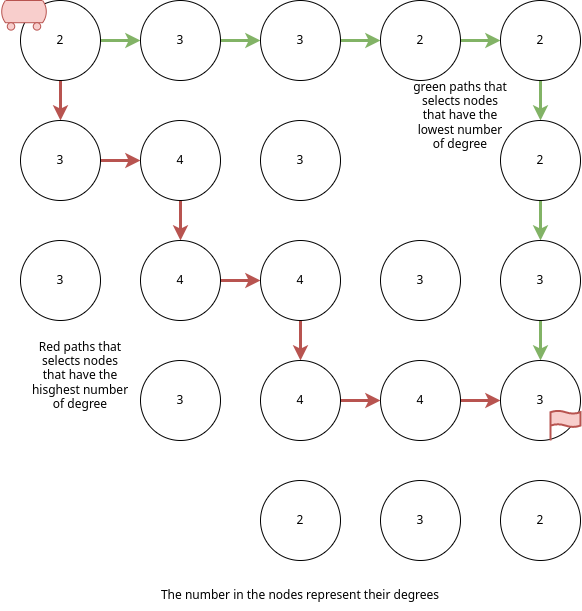
\includegraphics[width=\widthimg]{img/criteria_degree.drawio.png}
\end{figure}


\subsubsection{Coverage of the graph}\label{sec:graph_coverage}

Coverage of a graph represents the proportion of the graph that is used by an agent. We can define graph coverage as such: \[
  coverage(\pi) = \frac{|vertex(\pi)|}{|V|}
\] Graph coverage definition changes given the input; \[
  coverage(\gamma) = \frac{| \bigcup^{\pi \in \gamma} vertex(\pi) |} {|V|}
\] Finally, \[
  coverage(\tau) = \frac{| \mathlarger{\mathlarger{\bigcup}}^{\gamma \in \tau}{ \text{  } \bigcup^{\pi \in \gamma}{vertex(\pi)}} |} {|V|}
\] where \(vertex(\pi)\) is a function that returns the associated vertices set of the sequence of vertices.


\subsection{Selection of one path considering other agents}

\subsubsection{Path conflict}
Potential conflict represents a function counting conflict occurring between agents considering time step. It takes as input a set of path \(\tau\); formally we define first \[
    pc(\pi,\pi') =   \sum_{t}^{min(|\pi|,|\pi'|)}{
        \begin{cases}
            1   & \text{if  } conflict(\pi,\pi',t) \\
            0   & \text{otherwise}
        \end{cases}
    }
\] Where \(conflict\) returns the boolean value ``true'' if any conflict occurs between \(\pi\) and \(\pi'\) at time step \(t\), return ``false'' otherwise. Furthermore, \(pc\) does not forbid \(\pi\) and \(\pi'\) belonging to a same \(\gamma\).

We can then compare sets of paths:
\[ 
  pathc(\gamma,\gamma') = \mathlarger{\sum}_{\pi,\pi'}^{\forall \pi \in \gamma,\forall \pi' \in \gamma'}{
        pc(\pi,\pi')
    }
\] where \(\gamma\) an \(\gamma'\) are different sets of path, typically coming from \(\tau[a_{\in A}]\) and \(\tau[a'_{\in A}]\). We can then define \[
    PathC(\tau)= \sum_{a,a'}^{\forall a \neq a' \in A}{
        pathc(\tau[a],\tau[a'])
    }
\]

Another interesting function would be to compare a single path to a set of path \(\gamma\) or \(\tau\), indeed comparing all of the set of agents to all others, if their respective set of paths are large, the meaning of the comparison becomes blurry. We can in consequences define other functions that aims to keep interesting result not matter how much paths it takes as input:

\[ 
  pathc(\gamma,\pi) = \mathlarger{\sum}_{\pi'}^{\forall \pi' \in \gamma}{
        pc(\pi',\pi)
    }
\] and \[ 
    pathc(\tau,\pi) = \mathlarger{\sum}_{\gamma}^{\forall \gamma \in \tau}{
        pathc(\gamma,\pi)
    }
\]

Another point to mention is that the definition is not complete; if two paths have different length, a part of the bigger path will not be considered

\subsubsection{Blocking agent}\label{def:blocking_agent}
  An agent \(a\) is called a ``blocking agent'' towards \(a'\), or agent \(a\) is blocking agent \(a'\), if at time step \(t\), all the next vertices from \(\pi_a(t)\) to \(\pi_a(|\pi_a|-1)\) are included in the vertices from \(\pi_{a'}(t)\) to \(\pi_{a'}(|\pi_{a'}|-1)\), for instance see figure\ref{img:blocking_agent} where red agent, at time step 1, is blocking the blue agent. Formally we have: \
  \[
    blocking(\pi,\pi',t) = \begin{cases}
      true   & \text{if }  since(\pi,t) \subset  since(\pi',t) \\
      false  & \text{otherwise}
    \end{cases}
  \] (We read ``path \(\pi\) is blocking path \(\pi'\) at time step \(t\)"). Where the function \(since\) is define as:
  \[
    since(\pi,t) = \bigcup_{i=t}^{i \rightarrow |\pi|-1} \{\pi(i)\}  
  \] which represent the set of vertices in \(\pi\) from \(t\) until the end of the path .
  
  It is called  ``fully-blocking''  if  \(a\) is a blocking \(a'\) at time step 0 (also see figure\ref{img:blocking_agent}). 
\begin{figure}[H]
  \centering
  \caption{Example of blocking agent}\label{img:blocking_agent}
  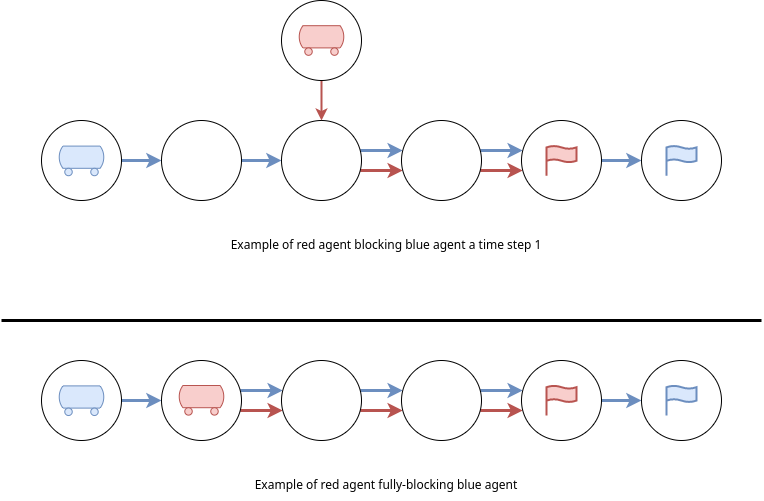
\includegraphics[width=\widthimg]{img/blocking_agent.drawio.png}
\end{figure}



\subsubsection{Potential conflict}
Potential conflict aims to count conflict occurring between paths without considering time step, in other words it delineate the union of common vertices between a all paths. it differs with path conflict by the fact that path conflict are defined according to time step, which is not the case for potential conflict. By definition, path conflict are specific cases of potential conflict, you can see as instance the figure~\ref{img:potential_conflict} which represent an isntance where no collision would occur, however there is a potential conflict represented by the yellow node. 

\begin{figure}[H]
  \centering
  \caption{Potential conflict}\label{img:potential_conflict}
  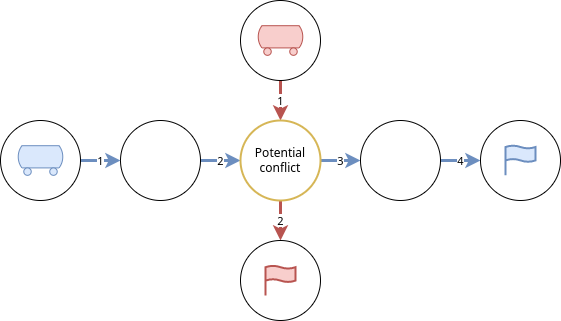
\includegraphics[width=\widthimg]{img/potential_conflict.drawio.png}
\end{figure} 

Formally, in order to define potential conflict, we have to define intermediate functions: \[
  potc(\pi,\pi') = |vertex(\pi) \cap vertex(\pi')|
\]
\[
  potentialc(\gamma,\gamma') = \mathlarger{\sum}_{\pi \in \gamma,\pi' \in \gamma'}{
    potc(\pi,\pi')
}
\]
\[
    PotentialC(\tau)= \sum_{a,a'}^{\forall a \neq a' \in A}{
        potentialc(\tau[a],\tau[a'])
    }
\]


We do not separate vertex conflict and edge conflict since it is by definition, included in the calculus; considering an edge conflict occurring a time step \(t\) (and \(t+1\)) between paths \(\pi\) and \(\pi'\), by definition, it means that \(\pi(t) =\pi'(t+1)\) and \(\pi(t+1) =\pi'(t)\). Thus, \(potc\) functions will count an edge conflict as two potential conflict. However, it could be interesting to separate potential edge conflict from potential vertices conflict.




% \subsubsection{Overused vertices}

% Overused vertices are vertices that are present in more than 

% \[
%   visited1^+(\tau) = \mathlarger{\mathlarger{\bigcup}}^{\forall a \neq a' \in A} (\forall\pi \in \tau[a] \cap \forall \pi' \in \tau[a']) 
% \]

\subsubsection{Conflict window}\label{sec:conflict_window}
A conflict window is defined with a couple of vertices \((v,v')\in V\) in a graph with orthonormal coordinate system, we also introduce the function \(coordinate:  V \rightarrow (\mathbb{N},\mathbb{N})\) which gives the coordinate associated to a vertex. Let \(C\) be a set containing all conflicts (these can be path or plan conflict), formally it can be define as \[
    C = \{v  | v \in V, conflict(v)\}
\] where \(conflict\) is a boolean condition; true if a conflict exist at vertex \(v\), else false. The next step is to ``draw" a rectangle (see \nameref{img:conflict_window} figure). To do so,  we use the the coordinates of vertices in \(C\) to construct this ``rectangle''. A conflict window is a set \(CW\) of vertices define as such: \[
  CW(C) = \{ v | v \in V, min_x(C) \leq x(v) \leq max_x(C), min_y(C) \leq y(v) \leq max_y(C)\}
\]

We described the approach to build one conflict window, however we can easily imagine building multiple by dividing the set of conflict into multiple subset. We however require that taken pairwisely, \(CW \cap   CW' = \emptyset, CW\neq CW' \); we could end-up with overlapping conflict window, which reduce the usefulness. The example in figure~\ref{img:conflict_window} shows four agents where three path conflict occurs. It also shows the resulting conflict windows; we can see that angles of the conflict window are not necessarily path conflict. 

\begin{figure}[H]
  \centering
  \caption{Conflict window}\label{img:conflict_window}
  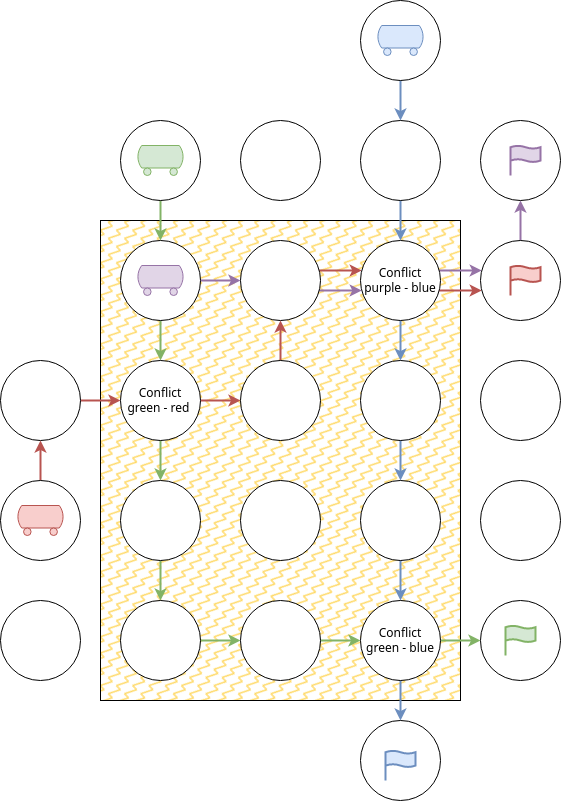
\includegraphics[width=8cm]{img/conflict_window.drawio.png}
\end{figure}


\subsubsection{Diversity}\label{sec:diversity}

Computing diverse path is mainly done using two different diversity measure; based on the Jaccard similarity coefficient (see \cite{habochal21a}), or on the the symmetry difference (also called Hamming distance) (see \cite{hanaka2022computing}) of two sets, we will respectively refer to them as \(diversity_j(\gamma)\) and \(diversity_{\bigtriangleup}(\gamma)\). Both compute diversity among two sets. The Jaccard similarity is defined as the size of the intersection of two sets divided by the size of the union of the two sets. In other words, it is a measure of how similar two sets are, based on the number of elements they have in common. we use them for computing diversity among two set of vertex issued from paths. The Hamming distance is a measure of the difference between two sequences of equal length. It is defined as the number of positions at which the corresponding symbols are different. The difference between the is that the Jaccard index focuses on the number of nodes that two paths have in common, while the Hamming distance focuses on the number of differences between the two paths. If we adapt the notation from the papers, we have
\[
  diversity_j(\gamma)=\sum_{\forall \pi,\pi' \in \gamma}{JaccardCoefficient(vertex(\pi),vertex(\pi'))}
\]

\[
  diversity_{\bigtriangleup}(\gamma)=\sum_{\forall \pi,\pi' \in \gamma}{SymmetryDifference(vertex(\pi),vertex(\pi'))}
\]  





\subsubsection{Distant}\label{sec:distant}
Let \(\gamma\) being a set of path of length \(n\), where all of the path have the same initial and ending position. Let \(\pi,\pi' \in \gamma\) two different paths. \(\pi\) and \(\pi'\) are considered ``most distant'' if no other path in \(\gamma\) have a higher distance. Distance between two paths is computed as such :


\[
  distance(\pi,\pi') = \sum_{k=0}^{n}{dist(\pi(k),\pi'(k))}   
 \] An intermediary function \(dist(V,V) \rightarrow \mathbb{N}\) is necessary; it represents an arbitrary distance function between two vertices, it can be the euclidean distance, length of the shortest path between them\ldots From \(distance\) definition, we can then define the distance from a path to a set of path \(\gamma\): \[
  Distance(\pi,\gamma) = \sum^{\pi'\in\gamma}{distance(\pi,\pi')}   
\] Considering then a set of \(k\) distant paths \(DP \subset \gamma \), \(\pi = pick(\gamma)\), \(\pi \notin DP \), \(\pi\) is distant towards \(DP\) (which means that if we add \(\pi\) to \(DP\), \(DP\) is still distant) if no \(\pi' = pick(\gamma), \pi' \neq \pi\) exist such as \( Distance(\pi,DP) < Distance(\pi',DP)\).


\subsubsection{Heatmap}\label{sec:heatmap}

Heatmap~\cite{atstfestko20a} is about projecting likelihood of presence of agents on vertices. Likelihood refers to the chance of an agent to be positioned at a specific vertex of the graph at a time step \(t\). We introduce the function \(\phi\) which compute likelihood of the vertex \(v\) at time step \(t\) for the set of path \(\gamma\) as such:

\[
  \phi(v, t, \gamma) = \frac{ |\{ \pi | \pi \in \gamma, \pi(t) = v \}|}{|\gamma| }
\]
  
From this definition, we can compute the first three step of an agent with an associated \(|\gamma|=3\) below (figure~\ref{img:heatmap}).

\begin{figure}[H]
  \centering
  \caption{Heatmap example of the first three time step for a \(|\gamma|=3\) }\label{img:heatmap}
  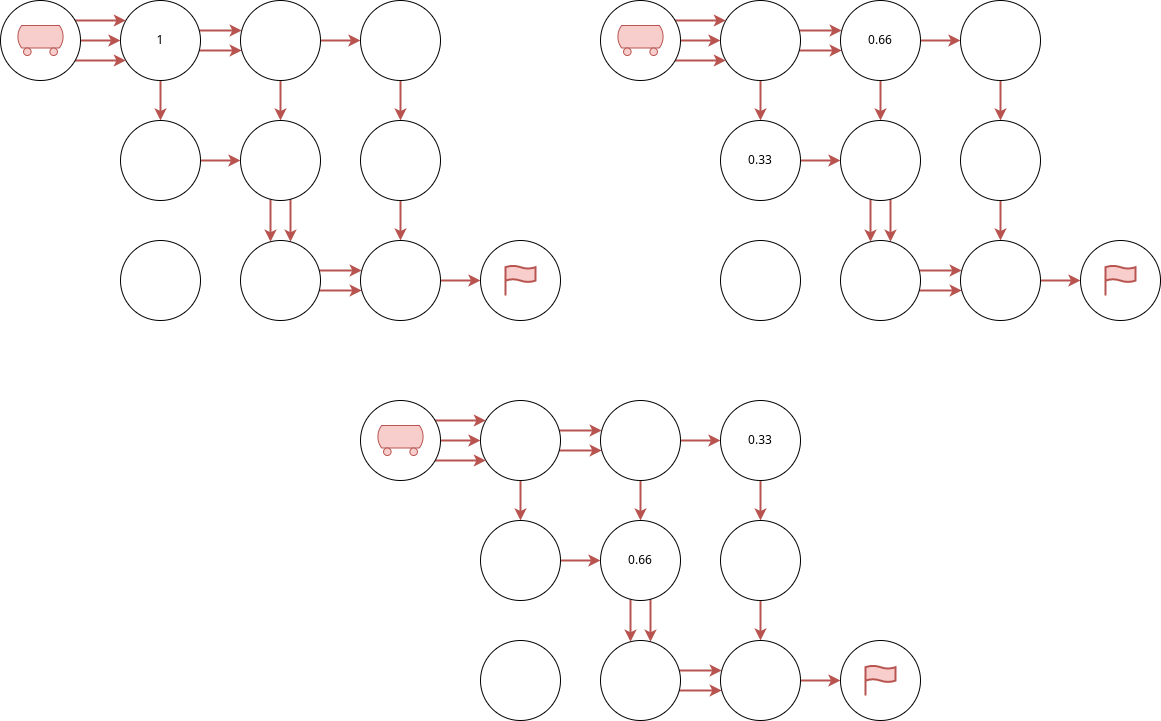
\includegraphics[width=10cm]{img/heatmap.drawio.png}
\end{figure}

This heatmap-per-agent can be used to compute a ``global one'', to do so, for each vertex and for each time step, we sum each \(\phi\) and then divide it by the number of agent (see appendix~\ref{apx:heatmap_and_global}), we will refer to this as \(\Phi\);

\[
  \Phi(v,t,\tau) = \frac{ {\sum^{\gamma \in \tau} }{\phi(v,t,\gamma)}}  {|\tau|}
\]



Computed this way, global heat maps no longer represent likelihood of presence, rather more an indicator. Both heat maps together can be useful for different parts of plan merging resolution.



The heatmap we proposed is from the perspective of agents, but it can also be considered with regards to the \(\gamma\)'s scope, especially paths and then, can become a property of a path. These likelihoods per paths gives us information one the path itself; having highs values represent that a vertex is used in different paths of \(\gamma\), a low average value represent a higher diversity and so on.

It becomes more interesting when we use these values as an objective function; allowing a maximum value for any \(\phi\) in an \(\gamma\) directly influence the way \(\gamma\) would be constituted; for instance, limiting the \(\phi\) value of a \(gamma\) for any vertex at maximum 0.4, forces the number of paths of at least three. Generally, the maximum or minimum value of \(\phi\) for any \(\gamma\) gives us information on how the paths are interacting.



% \subsection{Building interesting \(\tau\)}
% We defined different function that can represent properties of path in \(\tau\), however we can try to imagine set of path of different properties that makes \(\tau\) a ``better'' input for the merging section than a set of path containing a single property. We will start by trying to create interesting \(\gamma\), we will then discuss of the construction of \(\tau\).

% \(\gamma\) represent a set of path for a single agent, figure~\ref{img:building_gamma}~\cite{husvobbass22a,husvobbass22b} represent an instance where, if the blue path is the only one for the agent in \(\gamma\), finding a solution given orange and green path will require additional steps for the merging section, the idea of building an interesting \(\gamma\) is to provide at least both black and blue path. 

% \begin{figure}[H]
%   \centering
%   \caption{Example of providing two shortest path to provide solution}\label{img:building_gamma}
%   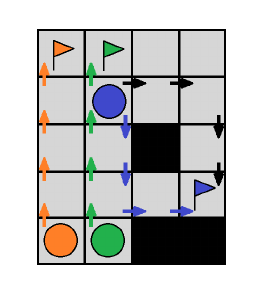
\includegraphics[width=\widthimg]{img/building_gamma.png}
% \end{figure}

% In the example~\ref{img:building_gamma} above, providing all the shortest path is ``easy'' (in terms of space search) how ever, on bigger instances, the number of possible shortest path is raising exponentially. Three approach can be used to build \(\gamma\).
% On the first hand, we can then imagine pre-defined \(\gamma\) requirements; as shown in figure~\ref{img:building_gamma}, black and blue path are two distant shortest path, furthermore, a set of three distant shortest path seems to be an interesting combination (see~\nameref{img:three_distant_path}, see~\cite{husvobbass22a,husvobbass22b}); the coverage of the graph (see~\nameref{sec:graph_coverage}) related to the number of path provided is quite interesting in low-obstacles density instances case, plus, by definition, the number of overlapping is guarantee to be the lowest given the number of distant paths.

% \begin{figure}[H]
%   \centering
%   \caption{Three distant path}\label{img:three_distant_path}
%   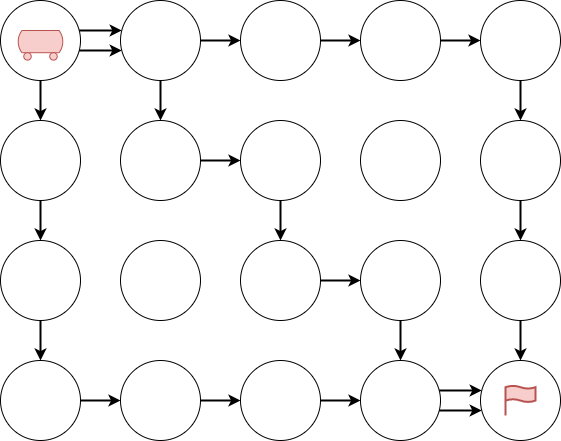
\includegraphics[width=\widthimg]{img/three_distant_path.drawio.png}
% \end{figure}

% Distant paths are part of the strategies provided in paper~\cite{husvobbass22a,husvobbass22b}, they also describe \textbf{Single path}, \textbf{All paths} which correspond to all the shortest path possible for an agent, \textbf{Random paths} which correspond to a subset of the previous strategy, furthermore the size of the subset is at most of size \(\frac{|SP|}{|SP^i|}\). The benchmark associated to the paper shows that the the Single Path strategy comes with the best result on both optimal and suboptimal strategies.

% On the other hand, we can automate \(gamma\) requirements through benchmarks and grid tuning; given a set of different cost function, we can determine which combination gives the best result by running tests on instances; number of instance solved, computation time, optimality...


\section{Merging}\label{sec:merging}
In this section we will define some approaches and heuristics in order to solve MAPF problems given a \(\tau\) input. The expression ``solving a conflict'' (or similar) will occurs, it however do not represent anything formal; it represent a moment where an approach has a solution to reach a vertex that is after the conflicting vertex, in the sequence of vertices \(pi\). Thus, it does not mean that no conflict may occurs because of the resolution.




\subsection{Sub-graphs}\label{sec:subgraphs}
Approaches in this section are using sub-graphs; one sub-graph is a graph based on \(G\) with the scope of a set of paths \(\gamma\); for every \(\gamma\) in \(\tau\) we have an associated sub-graph \(\mathcal{S}(\gamma)\). In others words, \(n\) agents result in \(n\) sub-graphs. For instance, let an agent \(a_{red}\) and \(a_{blue}\) with their set of paths \(\gamma_{red}\) and \(\gamma_{blue}\) where \(|\gamma_{red}| = 2\) and \(|\gamma_{blue}| = 1\). The result of the decomposition of \(\tau\) in sub-graphs is in figure~\ref{img:from_graph}. 

\begin{figure}[H]
  \centering
  \caption{Decomposition of \(\tau\) in sub-graphs }\label{img:from_graph}
  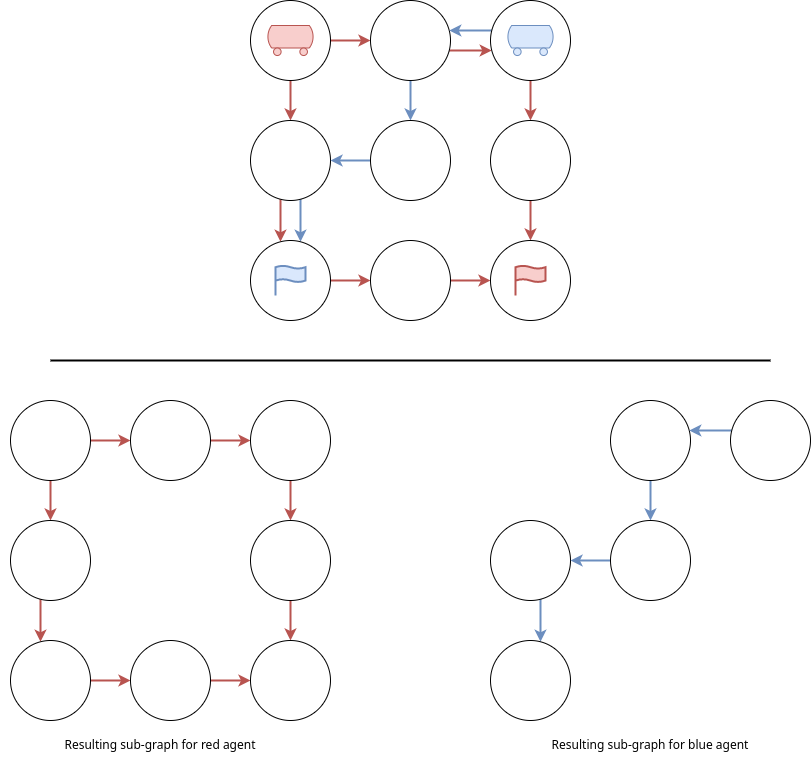
\includegraphics[width=\widthimg]{img/from_graph_to_subgraph.drawio.png}
\end{figure}

Sub-graphs by themselves are not useful, approaches can extend the sub-graphs according to strategies. Intuitively, an ``extension'' represent additional possibilities in order to solve a conflict. 

\subsubsection{Witness solver}

In this section, we will introduce a witness solver; a witness solver (WS) will be the basic solver that aims to solve MAPF instance given a \(\tau\) input. It works as such; it converts the input \(\tau\) in a set of \(n\) graph that are sub-graph of \(G\) as described in section~\ref{sec:subgraphs}. We then have two cases: there is a valid plan made out from \(\tau\) that contains no path-conflict, or there is no valid plan that can be build ot of \(\tau\) directly. In the first case, the merging process will give the valid plan as output, in the second case, the WS will try to solve the instance by using different approaches, strategies or heuristics until finding a valid set of paths that is a valid plan.

The first case occurs if it exists a set \(\{pick(\gamma) | \gamma \in \tau\}\) which correspond to a collection of path, is conflict-free, we refer to this case as ``straightforward solving''. However the process of picking these paths may be costly due to the exponential numbers of combination. We can use heatmap as a preprocessing work; from a global heatmap, we can directly tell from the paths if a straightforward solving is not possible if the following equation is true; 
\[ 
  \Phi(v,t,\tau) > \frac{ \sum^{\pi \in \gamma}{(1 \text{ if } v = \pi(t) \text{, else } 0)}}{|A|}
\] 
with \(|A| > 1\), for any vertex \(v\), at any time \(t\). The following figure~\ref{img:heatmap_sf_solving} shows an example where the straightforward solving is decided from the heatmap; the orange vertex as a \(\Phi\) value superior to \(3/4\) (issued from ). On the other side, the figure~\ref{img:heatmap_sf_solving_possible} show the opposite case.

\begin{figure}[H]
  \centering
  \caption{Example of instance that is not possible to use straightforward solving}\label{img:heatmap_sf_solving}
  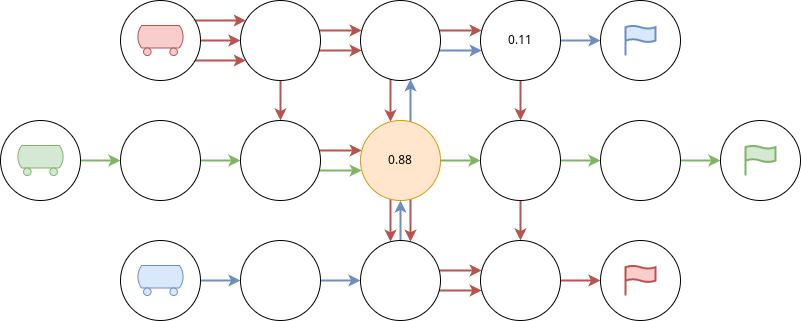
\includegraphics[width=\widthimg]{img/heatmap_sf_solving.drawio.png}
\end{figure}

\begin{figure}[H]
  \centering
  \caption{Example of instance that straightforward solving is at least undetermined}\label{img:heatmap_sf_solving_possible}
  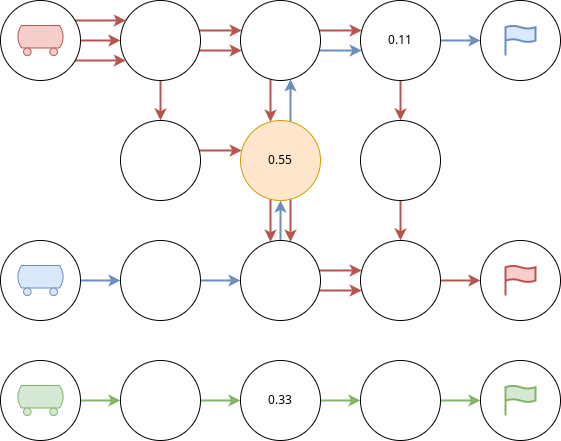
\includegraphics[width=8cm]{img/heatmap_sf_solving_possible.drawio.png}
\end{figure}

\subsubsection{Corridor}\label{sec:corridor}

The corridor approach aims to help the solving process by extending the size of the sub-graph generated by a set of path \(\gamma\). It extends the sub-graph by adding to the sub-graph the direct neighbor vertices (and their associated edges). Applying the corridor extension successively \(x\) times will result of a corridor of level \(x\) for instance:  
\begin{figure}[H]
  \centering
  \caption{Example of corridor}\label{img:corridor}
  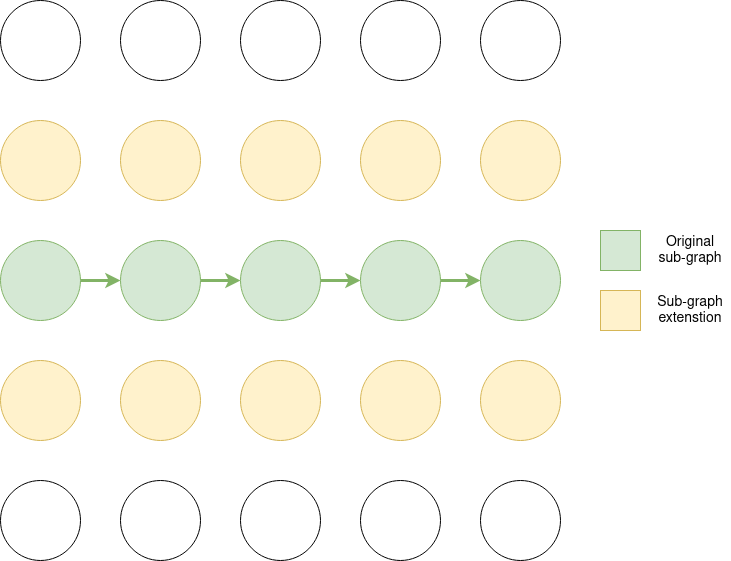
\includegraphics[width=\widthimg]{img/corridor.drawio}
\end{figure}

We can define corridor as such;

\[
 corridor(s,(V,E)) = \{v' | v' \in V, v\in s, (v,v') \in E \}
\] where s represent of set of vertices.

A corridor of \(k\)-level(s) is obtained by recursively use the corridor function \(k\) time on its output: e.g. \(corridor(corridor(vertex(\pi),G))\) represent a 2-levels corridor.
We can assume some elements about this approach; with a big enough \(k\) size the whole graph is covered. Using the witness solver would end up doing classic MAPF. Furthermore for large instances, a huge part of the extension would probably not be used ending up adding more space search for the witness solver. We can also identify instances where corridor extension would be probably interesting to use when the ``dodge'' movement required to solve a conflicts is situated in the graph ``far away'' (a distance relatively high) from where the conflict occurred. We can also assume that a set of distant paths would be an interesting set to work with; it potentially limits the number of ``overlapping'' vertices that would be added by the extension, see example shown in figure~\ref{img:case_corridor}. Also, corridors may work better on low density instances and low number of conflicts and potential conflict since it is not adding so much depth of possible movement.

In practice, we can create corridor only for path that have a path conflict, we can also choose to create corridor only for one of the two agent involved in a conflict.


\begin{figure}[H]
  \centering
  \caption{Most Distant paths and corridor extension}\label{img:case_corridor}
  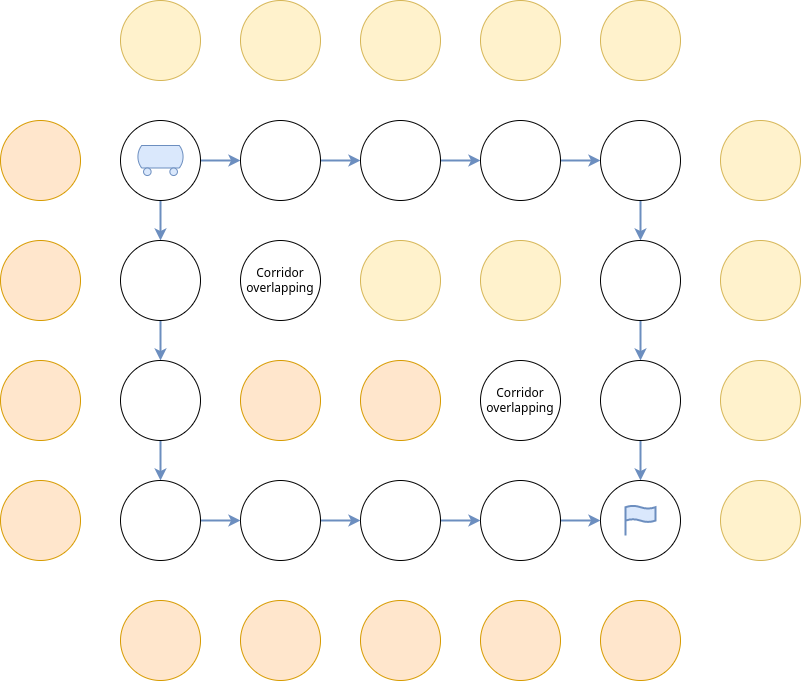
\includegraphics[width=\widthimg]{img/case_corridor.drawio.png}
\end{figure}


\subsubsection{Diamond extention}

The diamond extension aims to extend the sub-graph by adding diamonds of vertices around potential conflict or plan conflict. As shown in figure~\ref{img:diamond}, we can se different levels of diamond extension which will increase the size of the sub-graph, by extension the possibilities in order to solve the conflict.
\begin{figure}[H]
  \centering
  \caption{Example of diamond of size 1 and 2}\label{img:diamond}
  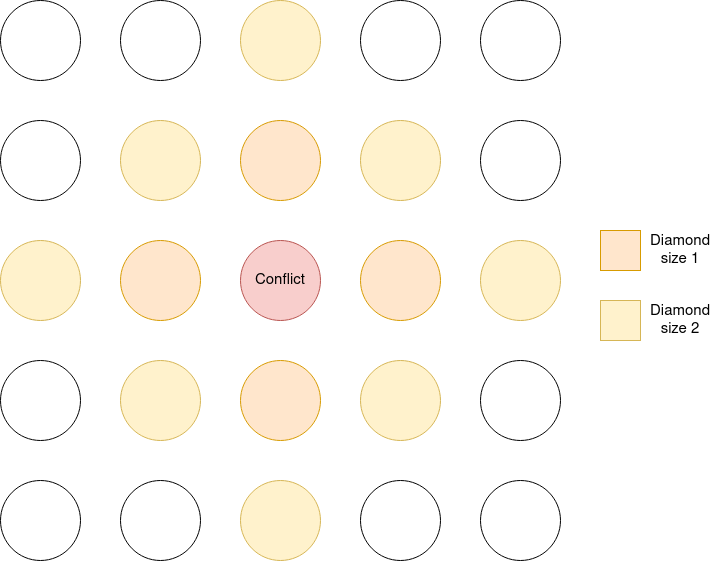
\includegraphics[width=\widthimg]{img/diamond.drawio.png}
\end{figure}

As described for the corridor instance, having a \(k\) as diamond size too big would end up covering the whole graph. This approach would probably works fine with a relatively small \nameref{sec:conflict_window}; having all conflicts concentrated in area of the graph would allow small size of the diamond extension, which reduce the space search. The instance represented in figure~\ref{img:diamond_case}, has a ``small'' conflict-window. While solving this instance (or this kind of instance, lot of robots, small conflict window) we can easily imagine that solving the conflicts issued by the IPF would create other conflicts but still in the same area. In consequences, diamond extension seems appropriate since the extension is covering also close area around conflicts. 
\begin{figure}[H]
  \centering
  \caption{Example of diamond extension interesting case }\label{img:diamond_case}
  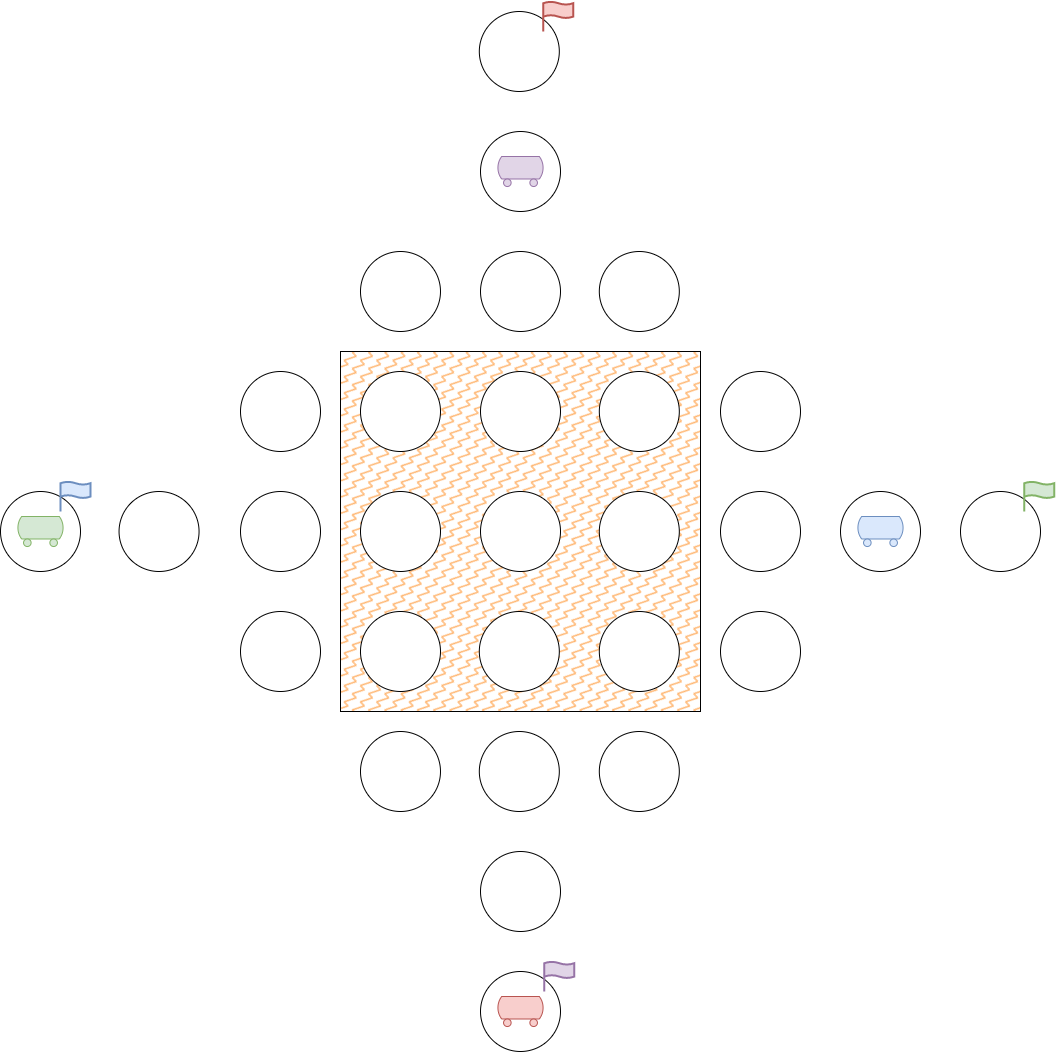
\includegraphics[width=7cm]{img/diamond_extension_case_example.drawio.png}
\end{figure}

From the properties described in section~\ref{sec:ipf}, we can argue that paths that have few bendings would work better for the diamond extension; a higher proportion of the extension (of size higher than 1) will already be in the original paths. Furthermore contrary to the corridor extension, whenever the proportion of conflict is low compared to the length of the path, diamond extension would probably work better e.g. figure\ref{img:diamond_vs_corridor}, based on section~\ref{sec:corridor} and figure~\ref{img:corridor} the proportion of the sub-graph that is not used is way higher for the diamond extension.

\begin{figure}[H]
  \centering
  \caption{Example of case where diamond extension would work but not corridor extension}\label{img:diamond_vs_corridor}
  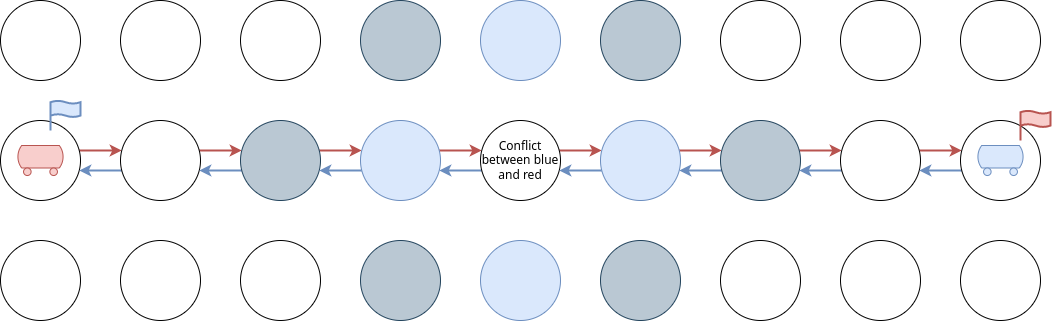
\includegraphics[width=\widthimg]{img/diamond_vs_corridor.drawio.png}
\end{figure}





\subsubsection{Systematic extention}

Approach presented above are not complete and aim to reduce the space search or computation time at the probable cost of optimality. Furthermore we can imagine instances where both approaches would not work, or require too much computation time. In the case represented on figure~\ref{img:systemetic_instance}, considering that \(\tau\) contains for both agent one shortest path, it is easy to tell that both heuristics on this kind of instances would not work decently because it would require that the extension covers the whole graph.

\begin{figure}[H]
  \centering
  \caption{Example instance that are more complex to solve}\label{img:systemetic_instance}
  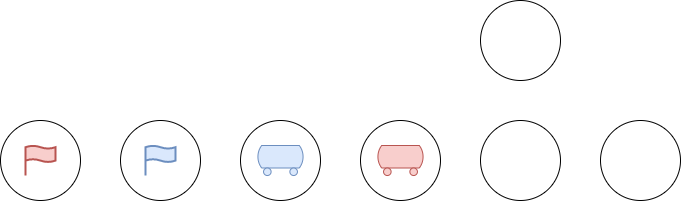
\includegraphics[width=\widthimg]{img/systematic_instance.drawio.png}
\end{figure}

We can use solving strategies described in paper~\cite{husvobbass22a,husvobbass22b}. These paper introduce four different strategies; Baseline Strategy,  Makespan-add Strategy, Prune-and-cut strategy and the Combined strategy. For short, these strategies are using a \(k-restricted graph\) which is similar to sub-graph; it takes a shortest path \(SP\) to define a subgraph, it also add ``vertices that are at most distance \(k\) away from some vertex in \(SP\)". The main idea is to add vertices and/or raise the makespan and see if a solution exist. According to the benchmarks, the Combined strategy seems to to most successful.

\subsubsection{Improving subgraphs with heatmaps}

An advantage of the subgraphs approach is that the approach can work till the subgraph contains the initial and final position and is connected. We can then, instead of increasing its size as we proposed before, prune part of the graph. To do so, we can aim specific vertices of the graph that can be identified using heatmap (see~\ref{sec:heatmap}). In a way, we can try to reduce \(\Phi\) values of the global heatmap by removing some vertices of subgraphs. We can imagine different criteria that would be deciding which vertex can, or should be pruned, for instance we can select vertex of the subgraph that has a high \(\Phi\) value but a low \(\phi\), in other words, removing vertices that are, for an agent not essential, but used by other agents.

On the other hand, heatmap can be used to tune the different approach we described before. For instance, we can apply bigger diamond extension on a vertex that have a conflict and a high \(\Phi\) value.  




% \subsection{Guiding the agents}

% We described above strategies working with sub-graphs, however we can use \(\tau\) in other way. Instead of creating subgraph, we can uses all of the paths in \(\tau\) to create a ``heatmap''. Heatmap describe where agents has the most probable position. To do so, we project the probability of presence on each nodes of the graph for each time step. We can define two types of heatmaps, a ``global heatmap'', which refer to the heatmap considering all agents. And one specific to an agent, called ``local'' heatmap, respectively, we have  \(Heat(\tau)\) and \(heat(\gamma_a)\). We can define local as such:

% \[
%  heat(\gamma) = 
% \]

% Global heatmap is made of all local ones; in other words, for each nodes of the graph, we sum the probability of presence for each agent, the total being divided by the number of agents. There is some properties that we can infer from the global heatmap: if a node has a joined presence probability \(P\) of 1, we can tell that \(\tau\) contains no selection of paths for each agent such as no conflict occurs. This event is a specific case of a more general definition:

% \begin{definition}
%   If there is a vertex  \(v \in V\) having a \(P(v) \geq  1-(1/|A|)\), where \(P(v)\) is computed given an input \(\tau\), it is not possible select a path \(\pi\) where \(v \in \pi\) for straight forward solving.   
% \end{definition}

% (need a proof)








% The approach of heatmap uses the different path in \(\tau\) to project on graph the probability of presence of an agent. The figure~\ref{img:heatmap} shows the heat map of a graph considering \(\tau\) with two agents; a red one with two paths and a blue one with one path. 



% Using these ``probability of presence'' we can select which path to select to, in this case reduce





% \subsubsection{Heatmap as a comparison tool}

% Global heatmap as we define it may also be a way to compare \(\tau\) together, respectively agent heatmap to another possible \(\gamma\) for a same agent. We can use a visual way to represent and compare different \(\gamma\) or \(\tau\). Even thought it it might not be the most reliable way, but it may be useful in order to fast compare multiple ones, for instance, the figure~\ref{img:colored_heatmap} shows how the complete figure~\ref{img:heatmap} (or the figure~\ref{apx:heatmap_and_global}) could look like with some coloration.  

% \begin{figure}[H]
%   \centering
%   \caption{Proposition of coloration for an agent heatmap, gradient from white (no presence), green (few presence) to red (high presence)}\label{img:colored_heatmap}
%   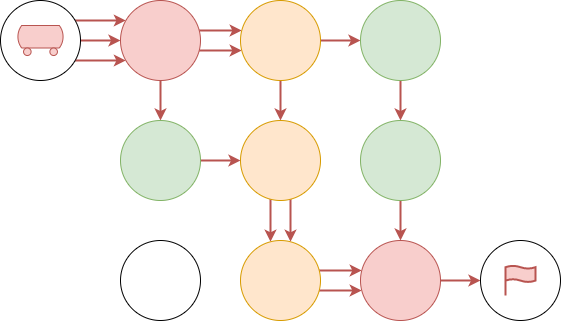
\includegraphics[width=\widthimg]{img/colored_heatmap.drawio.png}
% \end{figure}

% Furthermore, we formulate the following assumption \textit{``having a heatmap (global or agent one) that have the lowest sum of \(\phi\) and the lowest maximum \(\phi\) possible is desirable''} do not sound like a costly assumption. Given this assumption, we can then order different \(\gamma\) or \(\tau\) heatmaps. It of course, necessitate that the assumption is true, which may be (partially) decided with experiments.   


\subsection{Heatmap for subgraph}

\subsubsection{Straightforward solving}





\subsection{Heatmap as a solving strategy}


\subsubsection{Misc}



\begin{itemize}
  \item X Can help for making \(\tau\) ; The way we define \(\phi\) can be an objective function; trying to minimize the sum of every \(\phi\) 
  \item Comparing \(\tau\) ; It seems that it is a visual and easy way to compare two different \(\tau\), compare to other properties of paths that we defined, this one seems the most appropriate for comparison.
  \item Can help on the decision if the straight forward resolution is possible.
  \item Helping for the subgraph subgraph; we can remove part of the subgraph for some agent where the global heat indicator is high and sees if ot relax the problem or not (keeping a connected subgraph). It can also probably provide information on which vertex could be added instead
  \item Solving by Guiding the agent
  \item Suit easily for robustness
\end{itemize}




% 
\section{Misc}

\subsection{Going further on defining conflict}
We defined earlier that we would consider only edge and node conflict. Thus we can redefine them and add some variant; being able to have more information about a conflict might help us solving them or makes the selection of heuristics more robust (see~\ref{subsec:selecting_heuristic}). The first type of conflict hat we can identify is a conflict that can be solved using only wait move\footnote{It is of course not the only way, or even always the most efficient way of solving this kind of conflict} (see~\ref{img:waitconflict}). Formally, a  node ``wait-conflict'' \(c_{wait}\) occurs between agent \(a\) and \(a'\), if at time step \(t\),  \(\pi_a[t] = \pi_{a'}[t]\) and if \(\pi_a[t+1] != \pi_{a'}[t-1]\) and \(\pi_a[t-1] != \pi_{a'}[t+1]\). By definition, edge conflict can not be solved using wait only move. We can then consider the ``dodge conflict'', in contrary to the ``wait conflict'', ``dodge conflict'' can only be solved by extending the plan with unvisited node of the graph (in other words, extending the subgraph defined by a given path). Formally, node ``dodge conflict'' \(c_{dodge}\) occurs between agent \(a\) and \(a'\), if at time step \(t\),  \(\pi_a[t] = \pi_{a'}[t]\) and if \(\pi_a[t+1] = \pi_{a'}[t-1]\) and \(\pi_a[t-1] != \pi_{a'}[t+1]\). Edge conflict are by defnition ``dodge conflict''.

We can also identify reccuring conflict

Statment
\begin{itemize}
  \item Considering two paths of distinct agent, if they have more than 1 dodge conflicts, these paths are not shortest path. (I think)
  \item If two agents have dodge conflict, swapping their goals is an interesting move
  \item 
\end{itemize}






\begin{figure}[H]
  \centering
  \caption{Example of wait conflict and an example solution}\label{img:waitconflict}
  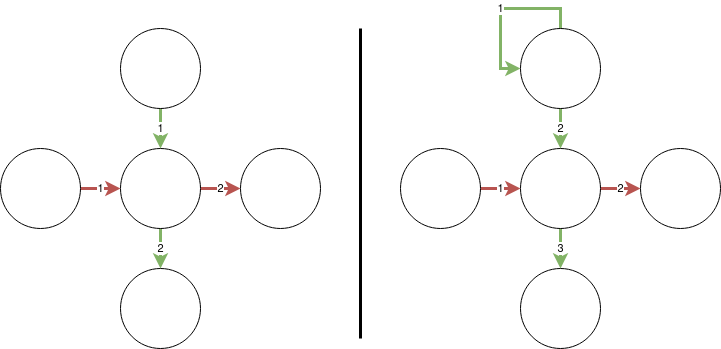
\includegraphics[width=\widthimg]{img/WaitConflict.drawio.png}
\end{figure}






\subsection{Selecting heuristic considering the MAPF problem}\label{subsec:selecting_heuristic}
Considering two MAPF problems \(A\) and \(B\), it is evident that a heuristic might be very effective for solving \(A\) but have no interest being used in \(B\). This can be due the graph (high/low density of obstacles, the size, etc), the number of agents, their disposition\ldots Hoever we can try to order or select the heuristics/approaches. Considering the reason enumerated above we can draw different metrics than might help selecting the heuristics/approaches:
\begin{itemize}
  \item Density of obstacles: can be computated by counting the average degree for each node of the graph.
  \item The size of the graph: can be computed by counting the number of nodes
  \item The disposition of the agents:\begin{itemize}
    \item We can count the number of groups that we can create (based on meta-agent technique or simple distance average selection)
    \item Average distance between agent (might need to be combined with a grouping techinque if agents a disposed at the edges of the graph)
  \end{itemize}
  \item Considering the kind of conflict
  \item others?
 \end{itemize} 

From the approaches that we defined, we can tell that corridor extention would not be selected if the density of obstacle is high (see~\ref{img:blocking_agent}).





\subsection{Others}
\subsubsection{Time expanded graphs}
Need to explore more about this; how it can help solving the problem, what are the kind of path that would be interesting as input, what merging strategies can be applied..

\subsubsection{Highway}
\begin{itemize}
  \item Summary: Highway\cite{coko16a,courkuxuayko16a} heuristic aims to change the graph by remove edges resulting with part of the graph that become oriented.
  \item Require: using following conflict paths might create better highway especially on self generated\cite{courkuxuayko16a} ones.
  \begin{figure}[H]
    \centering
    \caption{Example of highway (figure 2 of paper\cite{coko16a})}\label{img:highway}
    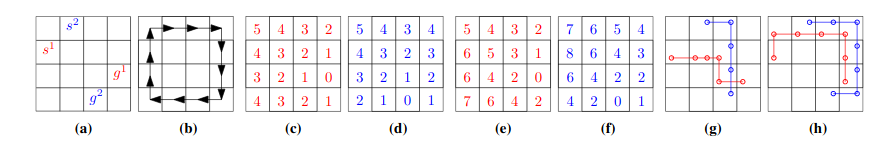
\includegraphics[width=\widthimg]{img/highways.png}
  \end{figure}
\end{itemize}


\subsubsection{Pruning by pulling goal}
\begin{itemize}
  \item Summary: Considering a agent and its path, each step both the goal and the agent are moving toward each other until a path or plan conflict occurs. Once a conflict is found, we use the position of the goal and the position of the agent to a rectangle (being the diagonal).
  \item Require: feels like it could only work for one path at the time, otherwise it might take too much computation time. 
  \begin{figure}[H]
    \centering
    \caption{Example of goal pulling}\label{img:pulling_goal}
    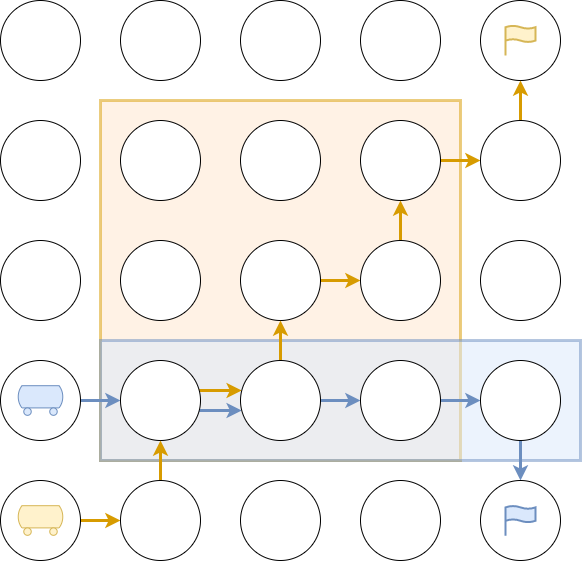
\includegraphics[width=\widthimg]{img/puling_goal.drawio.png}
  \end{figure}
\end{itemize}

\subsubsection{Loop Highway 14-Loyd-Puzzle, Carousel}
\begin{itemize}
  \item Idea: considering a path that goes through every starting position and goal position of every agents, loop, and do not cross; we can maybe assume that if the loop has two distinct conflict-free vertices neighboring the loop, their is a solution. If we consider that agent disappear on goal, it is an even better solution. If we can create the loop talked about above we are in a situation in worst case of the 14-Loyd-puzzle that I assume is solvable whatever the configuration. We can also consider multiple loops.
\end{itemize}

\begin{figure}[H]
  \centering
  \caption{Example of one loop and two loops}\label{img:loyd_loop}
  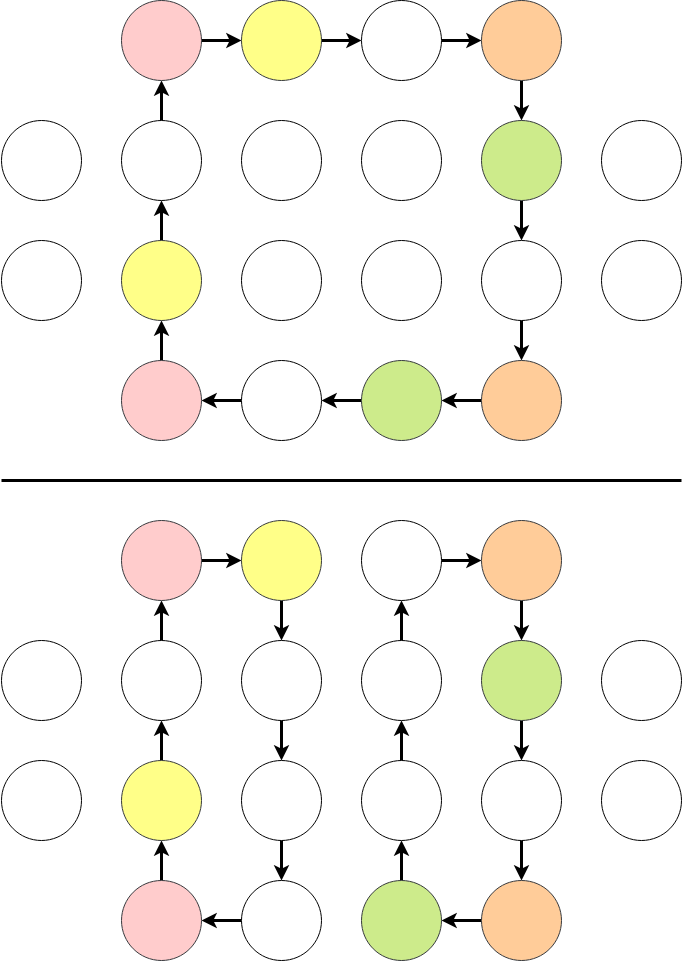
\includegraphics[width=\widthimg]{img/loop_highway.drawio.png}
\end{figure}

                             
\subsubsection{Waiting only}
\begin{itemize}
  \item Summary: the agents are only allowed to wait, no sub-graph extension is allowed.
  \item Require: In order to raise the chances of finding a solution, we need a higher number of diverse path, however, som problems can't  be solved through waiting, and some problem could be solved by waiting a huge amount of time. 
  \item Variant:\begin{itemize}
    \item Fixing waiting position with time interval\cite{phli11a,naphli12a}
    
    
    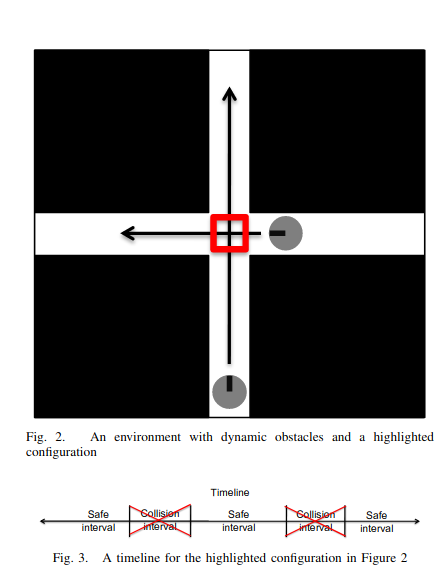
\includegraphics[width=5cm]{img/safeinterval.png}
    \item Fixing waiting position based on conflict free zone
  \end{itemize} 
\end{itemize}



\subsection{Guiding the agents}
\subsubsection{Heatmap}

\begin{itemize}
  \item Summary: The idea is to create for each vertices of the graph, an indicator that would describe how much the vertex ``used'' b y the agents. We can imagine something like, for each vertex, we have the number of time step where an agent is at the vertex divided by the makespan. The idea would then be to \begin{itemize}
    \item guide the agents using the indicator (the indicator may refer to the probability of presence of another agent)
    \item guide the graph extension by choosing the vertices that have a lower or higher ``usage''
  \end{itemize}
  \item Require: at least one path for each agents, the more paths we have the more precise the heat map can be.
  \item Variants: \begin{itemize}
    \item Take into consideration the robustness~\cite{atstfewabazh20a,atstfestko20a}
    \item make the heatmap evolve over time step
  \end{itemize} 
\end{itemize}



\subsubsection{From the bachelor thesis}
\begin{itemize}
  \item Deathlaser: the idea is to keep the agents at a closer position from their goal by pruning their subgraph around their previous position, probably require only 1 paths
  \item Homesick: the idea is to force the agent to come back to their plan after $t$ time not being on their original plan. Might require a graph extension beforehand 
  \item Checkpoints (or Divide and Conquer~\cite{yulav16a}): the idea is to add $n$ ``checkpoint'' vertices on the original path where their final paths should contains these vertices. Work only with one path 
\end{itemize}



\newpage
\section{Future work \& Conclusion}

To conclude, in this report we described and define what could be plan merging, starting by defining and formalize what are the two main part; Individual Path Finding and Plan Merging. We described for IPF various functions that could use as cost or objective functions in order to build interesting \(\tau\). Then we described different solving strategies that would take as input any \(\tau\). Multiple similar approaches and definition \cite{komenda2013repair,lichhadapeko22a} exists but do not obviously separate the two steps that I tried to define, which was my main objective.  

The whole report introduce different function, heuristics and strategies that could be implemented in order to be tested and benchmarked in future work(s). Furthermore, in the future, we would like to develop a framework which allows to visualize, test, and benchmark different IPF approaches, different \(tau\) building and merging strategies. 
In addition, due to the lack of time, multiple merging or solving strategies have not been explored such as ``guiding the agent via heatmap'', ``guiding the agent with time interval''\cite{phli11a,naphli12a}, taking into consideration robustness~\cite{atstfewabazh20a,atstfestko20a}, using highways~\cite{coko16a,courkuxuayko16a}. And finally explore the selection of strategies and heuristics given a MAPF problem instance. All of these topics are potential future addition to this report.
\newpage


\section{References}
\printbibliography[heading=none]

\section*{Appendix}
\begin{figure}[H]
    \centering
    \caption{Heatmap global and local}\label{apx:heatmap_and_global}
    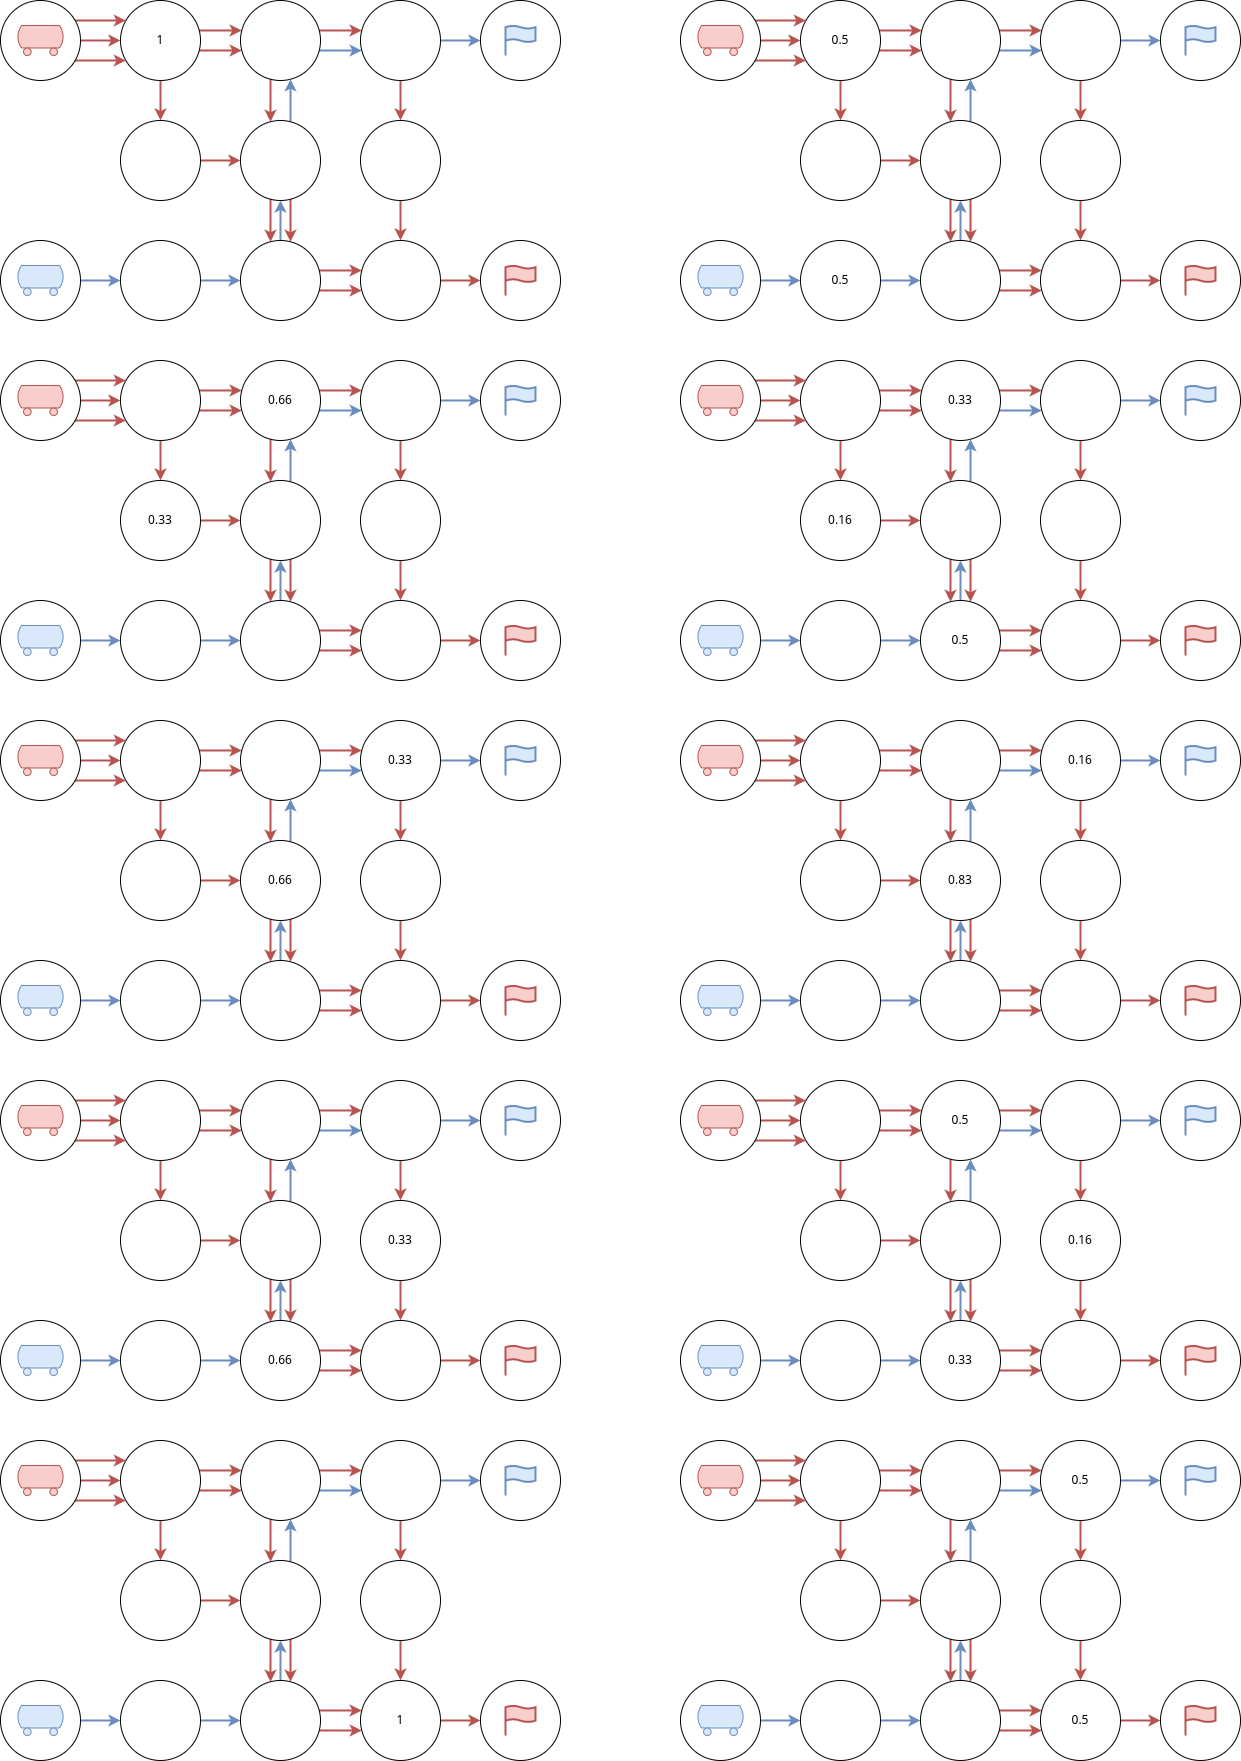
\includegraphics[width=12cm]{img/heatmap_and_global.drawio.png}
\end{figure}
\end{document}